\newpage
\section{Datenvisualisierung}\label{sec:Datenvisualisierung}
Die Visualisierung der aufgezeichneten Messwerte, so wie der ermittelten Zustandsbewertung des Systems soll über die Open-Source-Software Grafana erfolgen. Die Visualisierung der Daten soll hierbei nicht an die Zielplattform gebunden sein und von jedem beliebigen Rechner Abrufbar sein. Desweiteren soll die möglichkeit geboten sein, die Werte verschiedener Platformen in einem gemeinsamen Dashboard anzeigen zu lassen.\\
Das Konzept für eine Platformunabhängige Visualisierung der Hardware-Health-Monitoring Daten wird in Abbildung \ref{fig:DatenvisualisierungKonzept}. Hierbei werden die Daten der eizelnen Zielplattform einem Zentralen Server über eine REST \ac{api} in der Anwendung bereitgestellt. Der Grafana Service wird anschlißend von einem seperaten Server dem anwender bereitgestellt.   
\begin{center}
    \begin{figure}[h!]
        \centering
        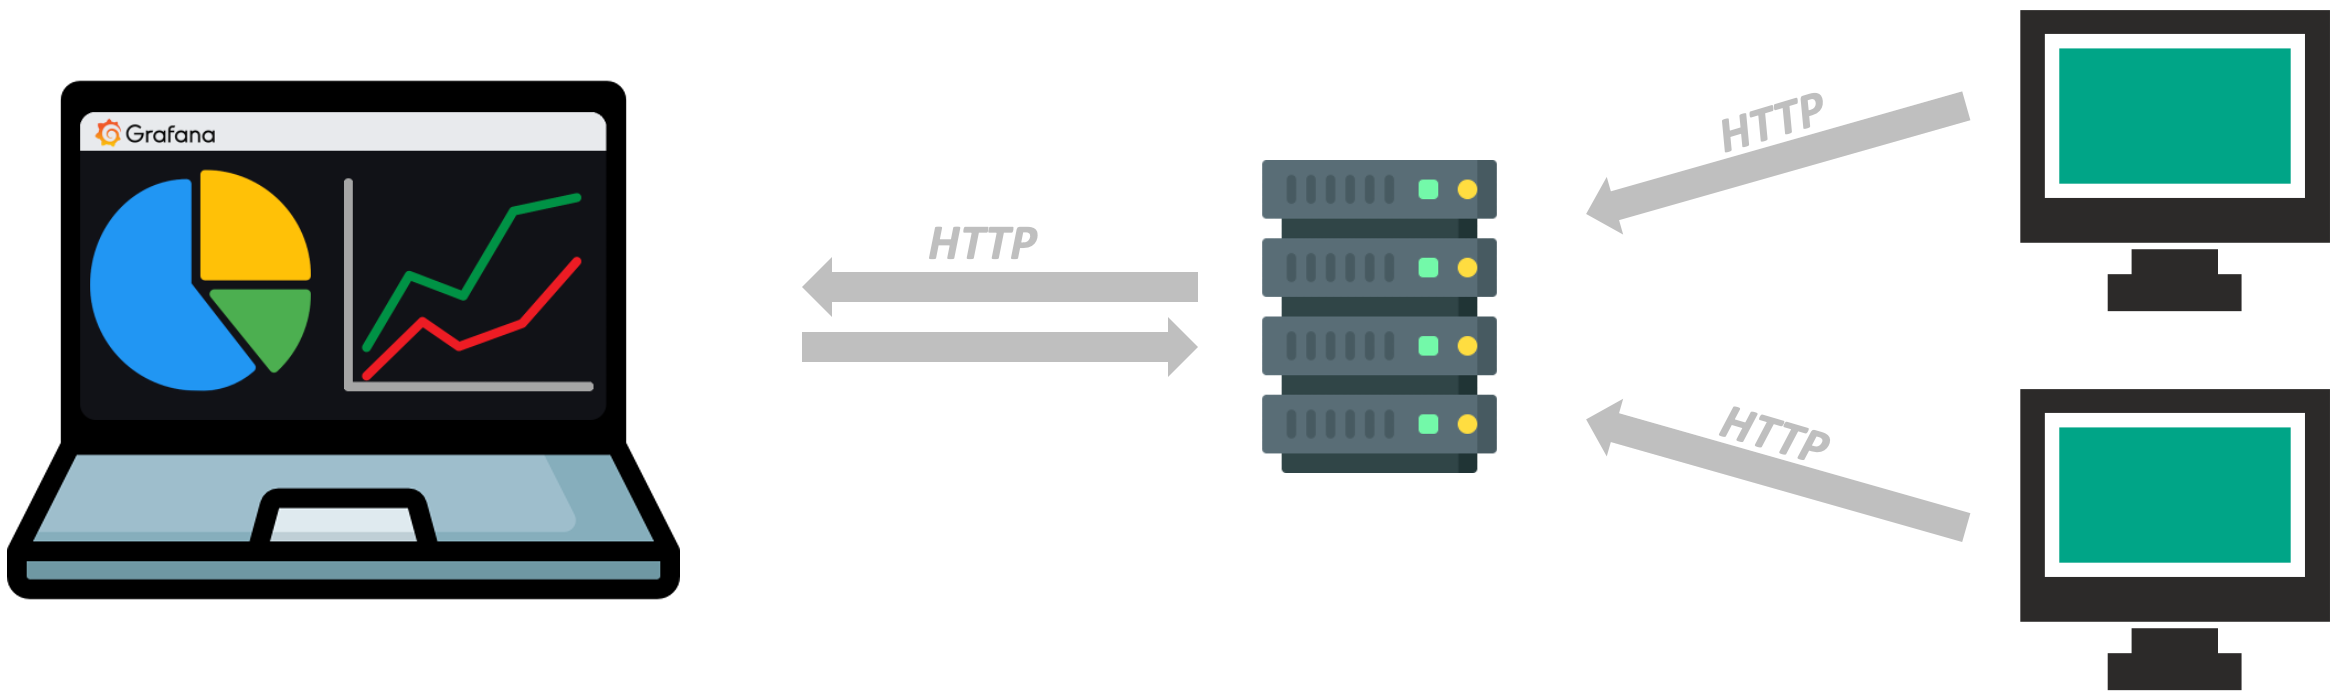
\includegraphics[width=1\textwidth]{Datenvisualisierung.png}
        \caption{Konzept zur Platformunabhängigen Datenvisualisierung}
        \label{fig:DatenvisualisierungKonzept}
    \end{figure}
\end{center}

\subsection{Architektur der REST API}
Die in Grafana verwendete Datenquelle \textit{SimpleJSON} diktiert die Struktur der \ac{api} vor. In der Dokumentation der Datenquelle \cite{SimpleJSON} werden die URL Pfade so wie Body der \acs{http} Anfragen erläutert.\\
Hierbei können, nach Abbildung \ref{fig:APIAnfragen}, die \ac{http} Anfragen an drei URL Pfade gesendet
 werden. Die URL mit dem Ende \glqq\textit{/}\grqq{} wird zum Testen der Verbindung genutzt. Anfragen an die URL \glqq\textit{/search}\grqq{} liefern eine Liste an vorhandenen Datensätze zurück. Diese wird genutzt um einen bestimmten Datensatz mit dem nächsten Aufruf der \ac{api} anzufragen. Über eine Anfragen an \glqq\textit{/query}\grqq{} können die gewünschten Datensätze erhalten werden.\\
\begin{center}
    \begin{figure}[h!]
        \centering
        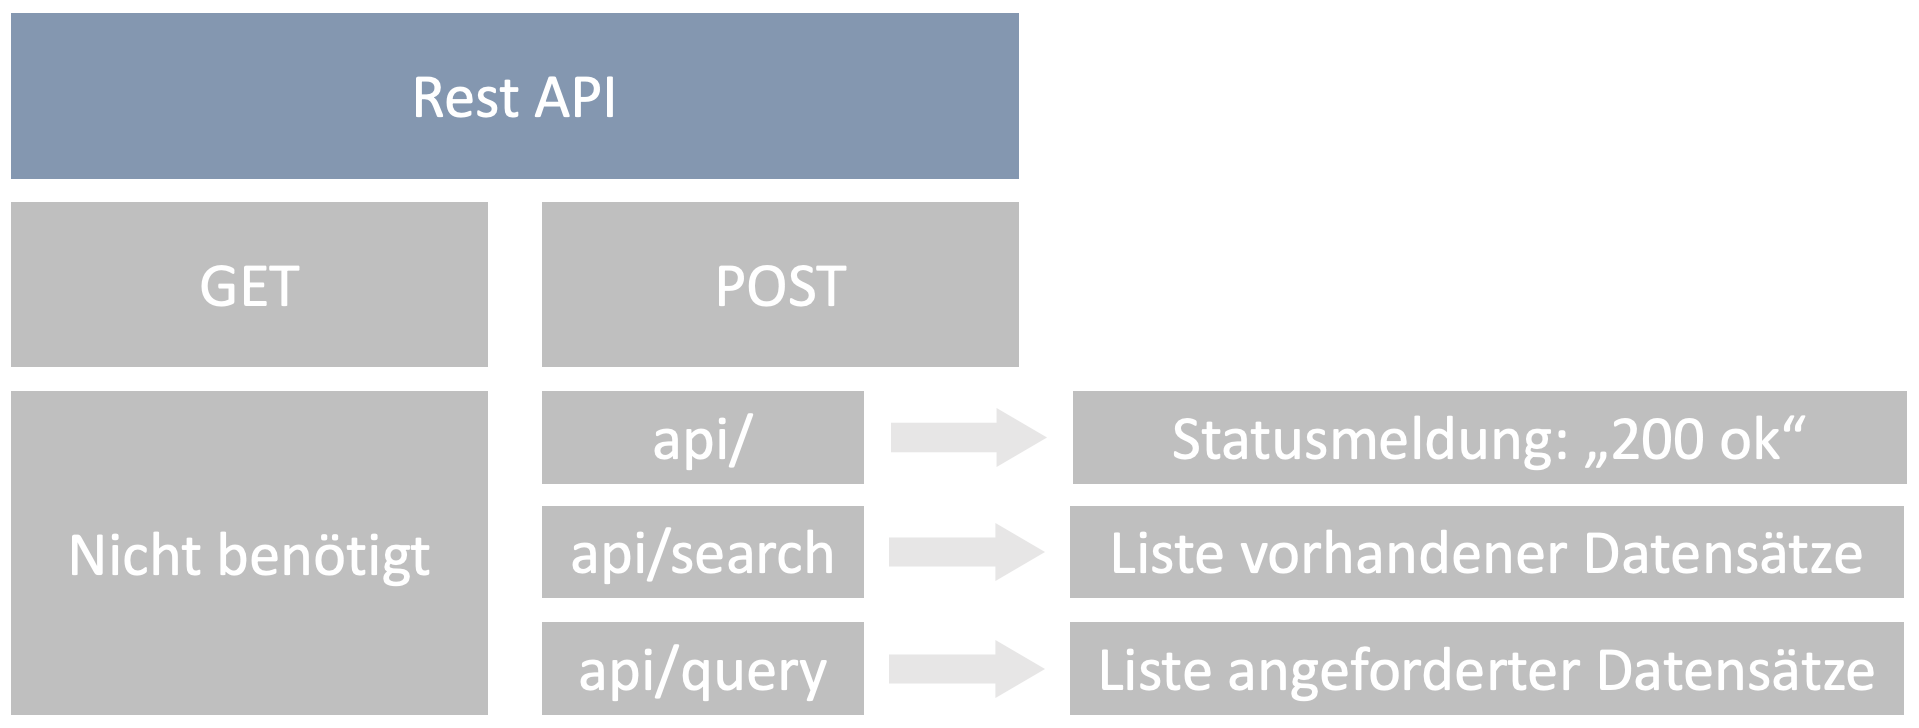
\includegraphics[width=1\textwidth]{APIAufrufe.png}
        \caption{Visualisierung der \ac{http} Anfragen an die \ac{api}}
        \label{fig:APIAnfragen}
    \end{figure}
\end{center}
\vspace{-1.8cm}
Da die Anfragen von Grafana in zufälligen intervallen gestellt werden, muss die \ac{api} zu jedem beliebigen Zeitpunkt auf diese reagieren können. Um wärend der behandlung einer Anfrage, nicht das gesamte Program lahm zu legen, wird die \ac{api} des Hardware Health Monitors in einem seperaten Thread gestartet und läuft unabhängig vom in Abschnitt \ref{sec:Gesamtkonzept} behandelten Taskscheduler.\\
Die \ac{api} wird in der Architektur der gesamten Anwendung von einer einfachen Klasse, welche unter dem Verzeichnis \textit{HM.API} organisiert ist, representiert. Abbildung \ref{fig:UMLAPI} zeigt zudem die verwendeten Resoursen der Schnittstelle. 
\begin{center}
    \begin{figure}[h!]
        \centering
        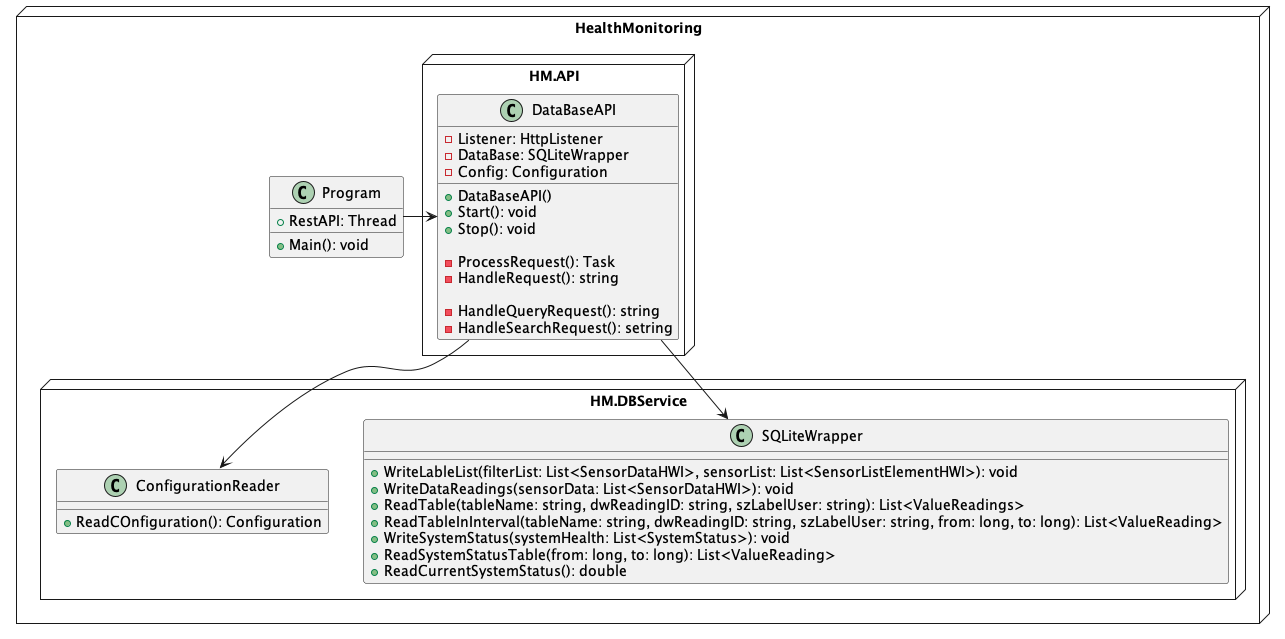
\includegraphics[width=1\textwidth]{DataBaseAPI.png}
        \caption{Arichtektur der \ac{api}}
        \label{fig:UMLAPI}
    \end{figure}
\end{center}
\vspace{-1.8cm}